\documentclass[11pt, oneside]{article}   	% use "amsart" instead of "article" for AMSLaTeX format
\usepackage[margin=0.75in]{geometry}                		% See geometry.pdf to learn the layout options. There are lots.
\geometry{letterpaper}                   		% ... or a4paper or a5paper or ... 
%\geometry{landscape}                		% Activate for rotated page geometry
%\usepackage[parfill]{parskip}    		% Activate to begin paragraphs with an empty line rather than an indent
\usepackage{graphicx}				% Use pdf, png, jpg, or eps§ with pdflatex; use eps in DVI mode
								% TeX will automatically convert eps --> pdf in pdflatex		
\usepackage{amssymb}

%SetFonts

%SetFonts

\usepackage{amsmath}
%\DeclareMathOperator{\mod}{mod}

\let\emptyset\varnothing

\newcommand{\reals}{\mathbb{R}}
\newcommand{\realsText}{$\mathbb{R}$}
\newcommand{\ints}{\mathbb{Z}}
\newcommand{\intsText}{$\mathbb{Z}$}
\renewcommand{\mod}{\ \mathrm{mod}\ }


\title{Correctness Quiz 1}
\author{Discrete Structures 2}
\date{21 February 2023, 9am}							% Activate to display a given date or no date

\begin{document}
\maketitle
%\section{}
%\subsection{}
\begin{center}
Name: \_\_\_\_\_\_\_\_\_\_\_\_\_\_\_\_\_\_\_\_\_\_\_\_\_\_\_\_\_\_\_\_ \\(please write legibly) 
\end{center}

\begin{enumerate}


\item Prove or disprove: 
Let $G=\langle L\cup R,E\rangle$ be an undirected bipartite graph with $|L|=|R|$. 
Suppose every node in the graph (that is, all nodes in $L$ and $R$) has at least one neighbor. 
Then the graph is connected. 
\vspace{10em}

\item Draw $\mathcal{K}_3, \mathcal{K}_4$ and $\mathcal{K}_5$. 
\vspace{15em}

\item Consider an undirected graph $G$ with $n$ nodes.
In terms of $n$, what is the longest \emph{simple} cycle that $G$ can contain? 
Give an example. 
\vspace{15em}

\item Identify a minimum spanning trees in each of the following graphs. 
If a minimum spanning tree does not exist explain why under the graph.
\begin{center}
\hspace{-3em}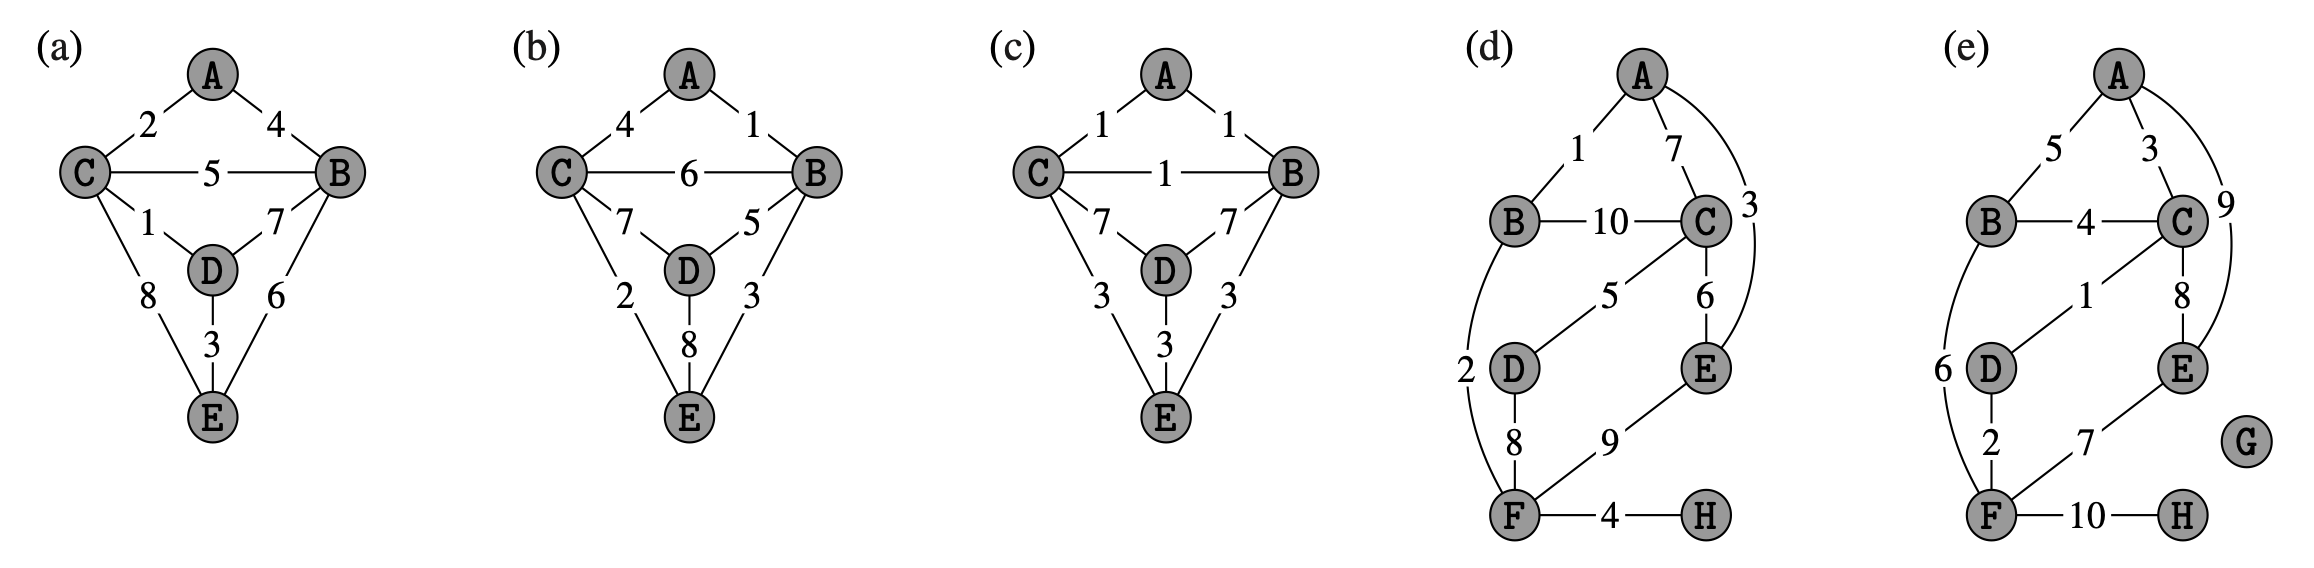
\includegraphics[width=\textwidth]{DS2-CH11-MST}
\end{center}

\item Match the term to its definition: 

\begin{center}
\begin{tabular}{lp{4in}}
\_\_\_\_\_\_\_ isomorphic & (a) a graph (or subgraph) where all possible edges are present between all nodes\\
\_\_\_\_\_\_\_ acyclic & (b) a graph such that it is possible to draw the graph such that no edges cross\\
\_\_\_\_\_\_\_ clique & (c) a graph that does not contain any simple paths between nodes and themselves\\
\_\_\_\_\_\_\_ planar & (d) two graphs for which there is a mapping between nodes and all edge relationships are equivalent \\

\end{tabular}
\end{center}

\end{enumerate}

\end{document}